


\begin{figure}[t]
\centering
  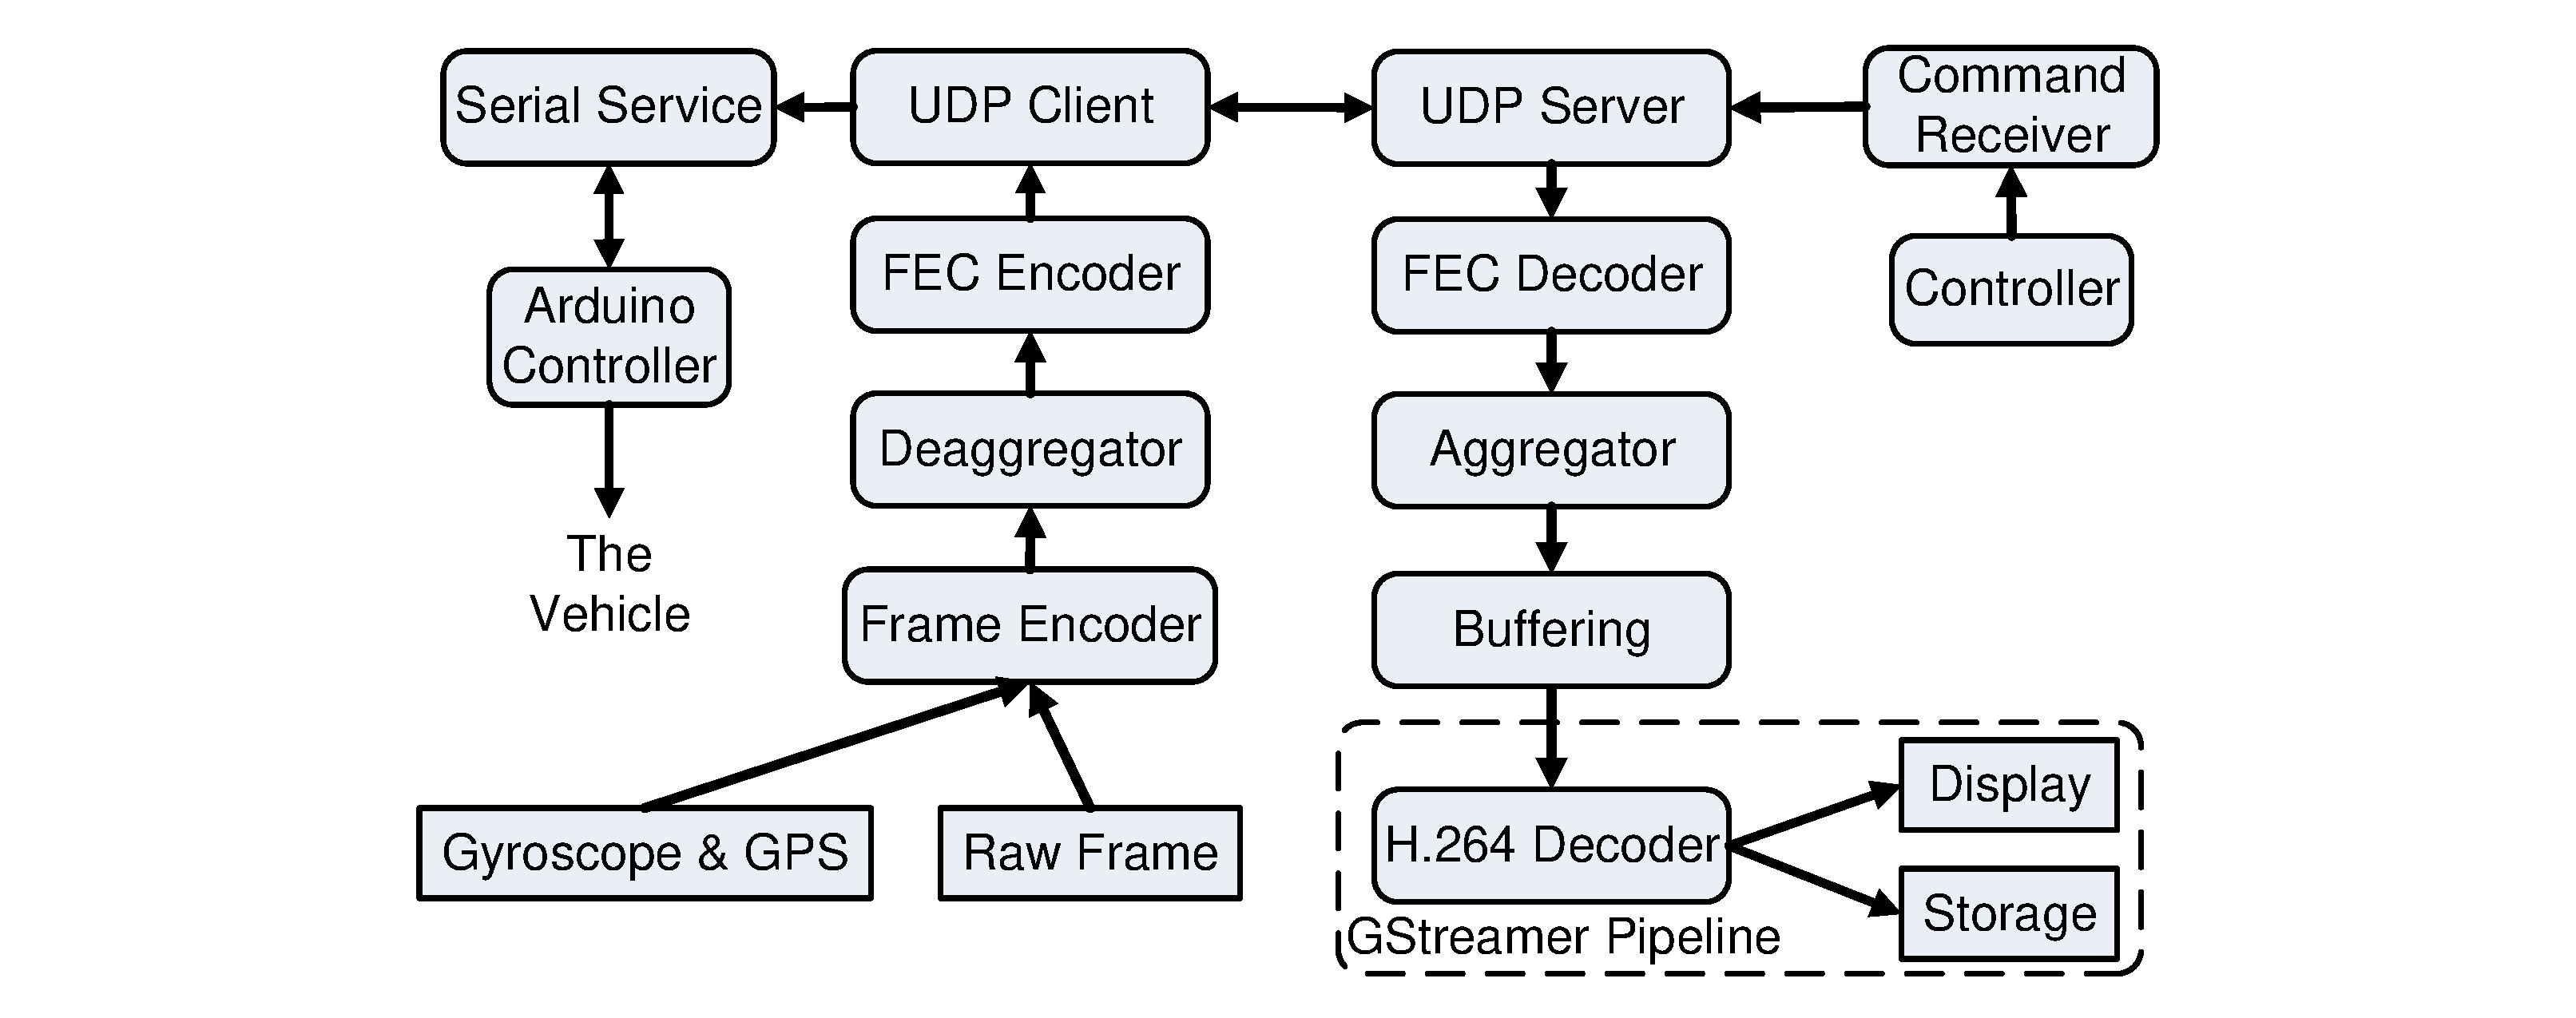
\includegraphics[width=3.4in,angle=0]{Figs/RTDrive/architecture.pdf}
\caption{The architecture of the live streaming and control system.}
\vspace{-0.5cm}
\label{server}
\end{figure}

RTDrive consists of an Android live streaming system and 
a remote control server. 
The architecture of the Android live streaming system is illustrated
in Fig. \ref{server}. 
The client side consists of two pipelines, the live streaming pipeline and the self-driving
pipeline. 
The live streaming pipeline includes context-aware video encoding, frame
deaggregation and FEC encoding.  
It encodes the video and streams to the remote server through transportation
protocols (details in section \ref{sec_udp_tcp}). 
The self-driving pipeline consists of object detection and lane marker detection. 
In the cases there is blockage in the lane, or no lane boundary is detected,
the control is transferred to remote server. 
while implementation of a fully self-driving vehicle
is out of the scope of this work, 
we present a framework that can be extended to a fully self-driving system, 
The architecture of the remote control server is illustrated in Fig. \ref{server}. 
It consists of two pipelines as well. 
A control pipeline is used to receive the control command from
an Android controller and then send to the vehicle. 
A video display pipeline is used to decode the frame packets
and display the streaming video to the operator. 



\begin{figure*}[ht]
  \begin{subfigure}[t]{0.32\textwidth}
    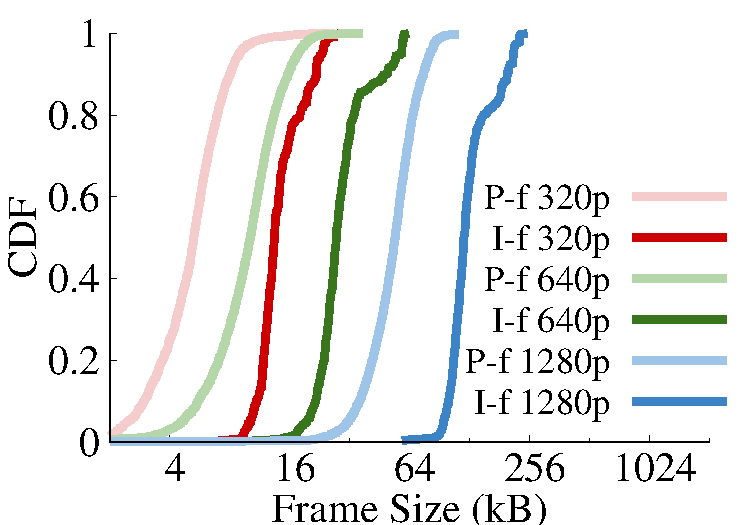
\includegraphics[width=\linewidth]{Figs/RTDrive/I_P_frame_size.pdf}
    \caption{The size distribution of I-frames and P-frames under three different resolutions and bitrates.}
    \label{frame_size}
  \end{subfigure}
\hspace{0.3cm}
  \begin{subfigure}[t]{0.32\textwidth}
    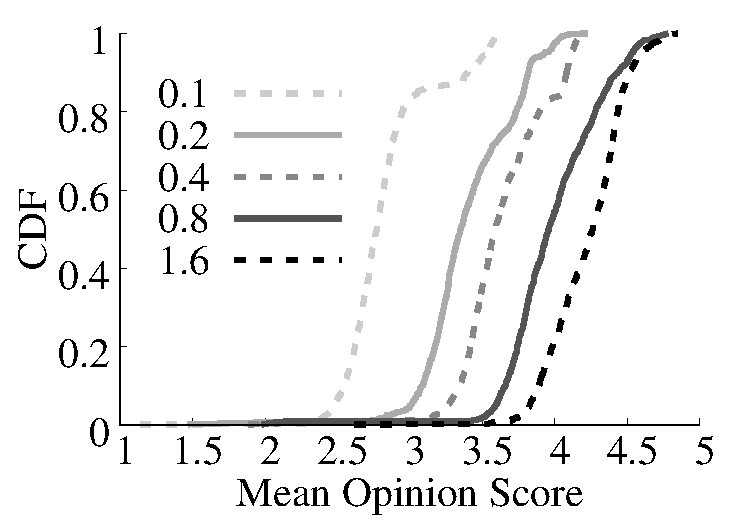
\includegraphics[width=\linewidth]{Figs/RTDrive/video_bitrate_quality.pdf}
    \caption{Video quality under different video bitrates (unit: mbps).}
    \label{bitrate_quality}
  \end{subfigure}
\hspace{0.3cm}
  \begin{subfigure}[t]{0.32\textwidth}
    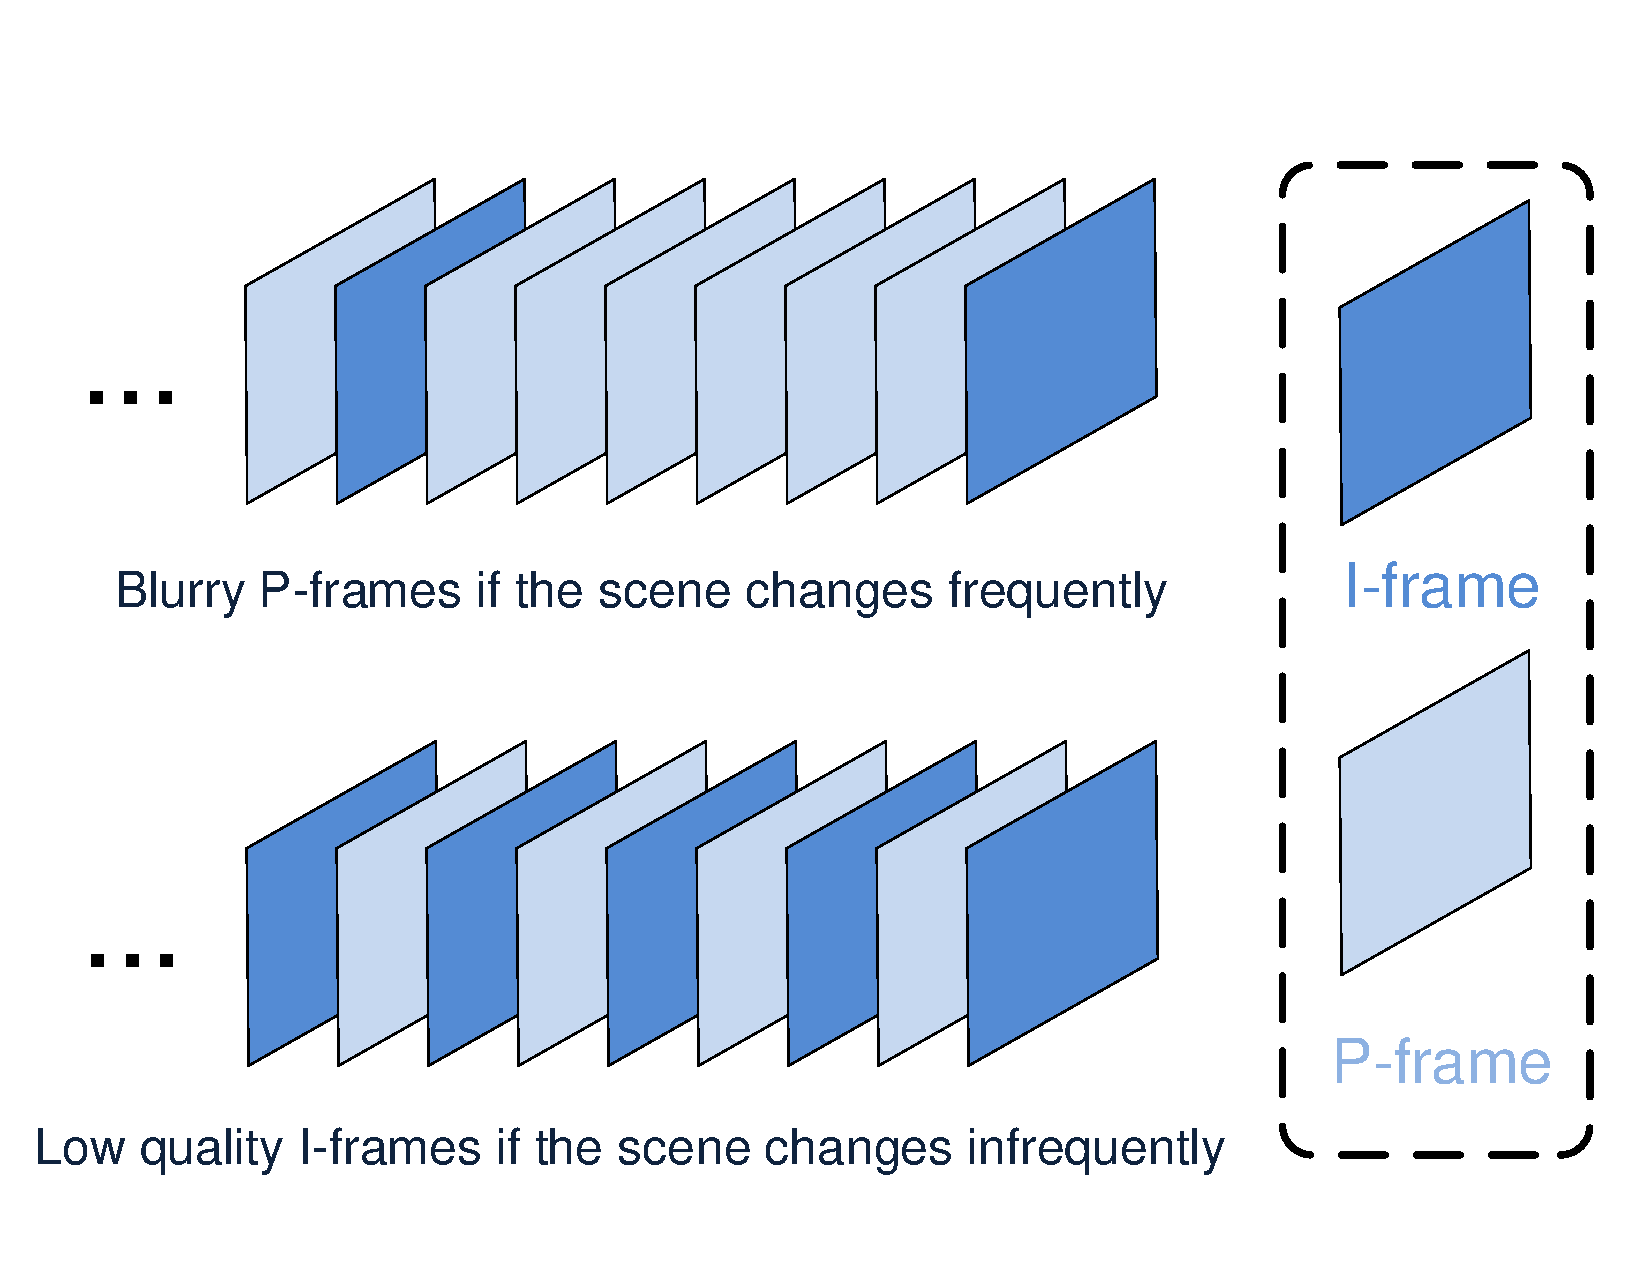
\includegraphics[width=\linewidth]{Figs/RTDrive/intervals.pdf}
    \caption{Illustration of I-frame interval and video quality.}
    \label{interval}
  \end{subfigure}
\caption{Video encoding and image quality.}
\end{figure*}


\subsection{Context-Aware Video Encoding}


Video encoding is a process that compress the raw video frames 
into frames of less sizes 
\footnote{Video/frame encoding is equivalent to video/frame compression 
and we use them interchangeably in this chapter}.
In this section, we present the overview of frame encoding, 
the relation between video encoding bitrate and video
quality, and how we can utilize
vehicle dynamics to improve video encoding efficiency.  

\subsubsection{Frame Encoding}
\label{sec_frame_encoding}




A video is a time series of video frames, or images. 
The size of each frame depends on the resolution and pixel encoding method. 
For example, for a frame of $w * h$ resolution, and each pixel 
is encoded by 3 bytes, i.e., 
one byte for each color of red, green and blue,
the total size of this frame is $3 * w * h$ bytes. 
For a frame with resolution of $640*480$, 
the size of one frame is around 1 Megabyte. 
The number of frames in one second is called frame rate. 
Suppose we send video streaming at 10 frames per second, 
we need a bandwidth of 100Mbps, which is too large to
be handled by today's wireless networks. 
Video streaming applications uses frame encoding techniques
to reduce the size of the frames. 
One frame can be compressed itself by using the statistical 
properties of image data. 
Continuous frames can be compressed by extracting the 
difference among video frames. 
The frame compression techniques can be lossless and lossy. 
Live streaming applications usually use lossy compression 
for its higher compression ratio. 


We compress the video by using video compression standard 
H.264 or MPEG-4 \cite{marpe2006h}.
In H.264, there are two types of frames, 
I-frame and P-frame. 
An I-frame, or Intra-coded frame, is a complete image. 
P-frame (Predicted frame)  
hold only the part that changes between frames.
The size distribution of I-frames and P-frames
under various resolution is illustrated in Fig. \ref{frame_size}. 
The three resolutions of 320x240, 640x480 and 1280x960, 
are set with bitrate 0.5Mbps, 1Mbps and 4Mbps, respectively. 
The size of I-frames and P-frames depends on 
the video encoding bitrate. 
If we use the same bitrate for two different resolutions, 
the frame sizes are similar but the quality will
be different (the relation between bitrate and video quality is
discussed in section \ref{sec_quality}). 
The median size of I-frames is 2-4 times larger
than that of P-frames in different resolutions. 
In other streaming applications, 
it can also use both previous and forward frames 
to generate B-frame (Bidirectional predicted picture) 
to better compress the frame.
B-frame is not used for live streaming as it requires
to stream the frame at the earliest possible time. 



The I-frame interval is defined as the time between 
two continuous I-frames and it is usually 1-5s \cite{zhang2012profiling, yu2014can}. 
The frame rate ranges from 1 to 15 in popular VoIP 
applications such as Skype \cite{zhang2012profiling} and Google Hangout \cite{yu2014can}. 
The server decompresses the video frame by using GStreamer pipeline \cite{gstreamer} 
and sends back the timestamp associated with the frame 
(the details are discussed in section \ref{streaming_protocol}). 


\subsubsection{Video Quality}
\label{sec_quality}


We use Blind and Referenceless Image Spatial Quality Evaluator (BRISQUE) 
\cite{mittal2012no} and Mean Opinion Score (MOS) \cite{bauman2017towards}
to evaluate the video/frame quality. 
The video quality is shown as a cumulative distribution function of frame qualities.  
BRISQUE trains a model using identical predictable statistical features, 
called natural scene statistics (NSS). 
NSS are based on normalized luminance coefficients in the spatial domain, 
and are modeled as a multidimensional Gaussian distribution. 
Distortions appear as perturbations to the Gaussian distribution.
It has been shown that these features correlate well with 
human judgements of quality \cite{mittal2012no, bauman2017towards}. 
The function uses the NSS features and corresponding opinion scores to train
a support vector machine regression model. 
The correlation between BRISQUE and MOS is summarized in Table \ref{brisque}.
It maps the score of one frame (0-100) calculated by BRISQUE to 
a MOS between 1 and 5. 
We use MOS as the only metric to evaluate frame quality. 

The video of one resolution can be encoded into different bitrates. 
High bitrate leads to high quality video. 
We compress a video with different bitrates (1kbps to 2mbps) and evaluate the video qualities.
The results are shown in Fig. \ref{bitrate_quality}. 
The bitrates of lower than 0.1mbps and higher than 1.6mbps are not shown 
in the plot. 
There are 1 I-frame within 10 frames 
and the 10\% of the frames with higher quality are mainly I-frames.  
Encoded video with lower than 0.1mbps downgrades the video quality marginally
comparing with the video with 0.1mbps. 
Similarly, encoded video with higher than 1.6mbps improves the
video quality marginally comparing with the video with 1.6mbps. 
Within the bitrate range of 0.1mbps and 1.6mbps, 
it roughly need to double the bitrate to improve the video quality linearly. 
We refer video encoding efficiency as the median video quality under
same encoding bitrate or the bitrates required to achieve the same
median video quality. 



\begin{table}[t]
  \centering
  \caption[psnr]{BRISQUE vs MOS}
  \vspace{-0.0cm}
  \label{brisque}
  \begin{tabular}{|c|c|c|c|c|c|}
  \hline
BRISQUE & 90 & 72 & 54 & 36 & 18
\\  \hline
MOS & 1 & 2 & 3 & 4 & 5
\\  \hline
Video Quality & Bad & Poor & Fair & Good & Excellent 
\\  \hline      
  \end{tabular}
  \vspace{-0.0cm}
\end{table}


\subsubsection{Context-Aware Encoding}


We present how to adjust video encoding parameters to improve
encoding efficiency according to vehicle dynamis in this section.
Suppose we use a fixed bitrate to encode a video, 
it is import to decide how many I-frames we want to encode. 
If the scene changes frequently, it needs more I-frames to reduce
the quality of each I-frame but increase the overall quality,
given the encoding bitrate is the same. 
If the scene changes infrequently, it needs less I-frames
to achieve a high encoding quality of I-frames 
as well as the P-frames since P-frames requires less data. 
An illustration is shown in Fig. \ref{interval}.
Our context-aware encoding technique utilizes this 
intuition to improve the overall video encoding efficiency
by sensing vehicle dynamics. 
The basic idea is to increase the I-frame interval at lower
speed and decrease it at higher speed or during steering events. 


To track the vehicular speed and angular velocity, we use
the GPS and the gyroscope sensor. 
The gyroscope is used to track 3D angular velocity of the 
smartphone. 
Interested readers can refer to \cite{wang2013sensing, chen2015invisible}
for how to use gyroscope to track vehicle steering events. 
The pseudo code of the context-aware encoding algorithm 
is shown in Algorithm \ref{contextaware}.
The $timestamp\_$ tracks the timestamp of last frame. 
the $gps\_$ and $gyro\_$ track the GPS data and gyroscope data 
recorded in last function call, respectively.
The $dist\_$ and $deg\_$ are the accumulated distance
and degree the vehicle travelled, respectively.
The $check\_$ refers to the checkpoint where last I-frame is created.
The algorithm checks the accumulated distance, angles and time
to decide if next frame should be I-frame or P-frame. 

%\begin{enumerate}
  \begin{algorithm}[t]
   \caption{Check if I-frame is required by sensing vehicle dynamics}
    \label{contextaware}
    \begin{algorithmic}[1]
\Function{requireKeyFrame}{$gps, gyro$}
  \State $now = currentTimeMillis()$
  \State $init = false$
  \If {$timestamp\_ == -1$}
    \State \Return $init = true$
  \Else
    \State $dur = now - timestamp\_$
    \State $dist\_ = dist\_ + gps\_.speed() * dur$    
    \State $deg\_ = deg\_ + gyro\_.angular() * dur$
  \EndIf
  \State $timestamp\_ = now$
  \State $gps\_ = gps$
  \State $gyro\_ = gyro$
  \If {$init || dist\_ >= \theta_{dist} || deg\_ >= \theta_{degree} || now - check\_ >= \theta_{t}$}
    \State $dist\_ = 0$
    \State $deg\_ = 0$
    \State $check\_ = now$
    \State \Return $true$
  \Else
    \State \Return $false$
  \EndIf
\EndFunction
\end{algorithmic}
\end{algorithm}
%\end{enumerate}



\subsection{Live Streaming Protocol}
\label{streaming_protocol}


We present the design of live streaming protocol in this section. 
We discuss different protocol design choice and present a consistent-latency
view when displaying live streaming video to remote operator. 
Measuring the performance of live streaming applications, such as 
Skype \cite{zhang2012profiling} and Google Hangout \cite{yu2014can}, 
is a active research topic. 
The implementation and application scenario differentiate us from
these measurement studies. 


\subsubsection{UDP or TCP}
\label{sec_udp_tcp}

Existing VoIP applications rely on UDP extensively, 
i.e., Skype \cite{zhang2012profiling} and Google Hangout \cite{yu2014can}.
Google Hangout uses UDP by default and switch to TCP if UDP traffic 
is blocked. 
Comparing with TCP, UDP is connectionless, does not have 
congestion control and retransmission mechanisms. 
In TCP, if one packet of a frame gets lost, 
packet frame will be re-transmitted and 
the frame is delayed for an entire RTT. 
In UDP, if one packet of a frame gets lost, 
the rest of the frame can be displayed and 
it does not introduce extra latency. 
Therefore, UDP is a better choice for live streaming
applications. 
However, if the UDP packet is lost, the video quality
will drop, 
so it usually comes with loss rate estimation and 
forward error correction mechanisms. 
In our framework, we implement both TCP and UDP
to understand and compare the performance difference.
In our UDP implementation, we use frame ACK 
mechanism to send back loss rate and bandwidth
estimation results to the live streaming system. 
The frame ACK is sent through the same UDP channel. 
We will discuss how to handle lost frame ACK
when estimating loss rate and bandwidth in section 
\ref{sec_lossrate} and \ref{sec_bandwidth}. 
In our TCP implementation, we use socket buffer size 
to estimate TCP transmission rate and adjust
video encoding rate at application layer. 
If there is packet loss in the network, the TCP connection
will reduce transmission rate and the application layer
will reduce video encoding rate. 


\subsubsection{Forward Error Correction (FEC)}
\label{sec_fec}

To improve the video quality upon packet losses, 
we introduce forward error correction (FEC) in our framework. 
Missing frame data may cause video distortion and flickering.
FEC, also known as eraser code, is widely used in wireless transmission \cite{yu2014can}
and reliable file storage \cite{plank2009performance}.
In FEC, each frame is encoded into $n$ packets of length $m$. 
Among the $n$ packets, the first $k$ packets are the raw data
of the frame, and the rest $n - k$ packets are encoded packets, 
i.e., each byte of the encoded packet is the linear combination 
of corresponding byte in the raw packets. 
Since each video frame has different size, $k$ and $n$ are 
different for different video frames. 
To encode and decode one frame, 
it requires the packets have the same length.
We use a reference packet length to estimate the $k$ first, 
and then assign each packet with equal length $sz / k$, 
where $sz$ is the frame size. 
In this case, we need at most $k$ bytes for the
padding of the last packet. 
It reduces the extra padding from $O(m)$ to $O(k)$ ($k$ is usually much smaller than $m$).  
In case of packet loss, $n - k$ packets are encoded as redundancy.
We define the redundancy ratio as $rr = (n - k) / n$. 
If any $k$ of $n$ packets are received at the receiver side,
then the frame can be recovered. 

\subsubsection{Loss Rate Estimation}
\label{sec_lossrate}

To decide how many packets to encode, we need to track
the loss rate of the UDP transmissions. 
On the server side, we calculate frame packet loss rate. 
To determine the number of data packets $k$ and that of coded packets $n$
to be included in a given frame, we
calculate the effective loss rates $L$ after the diversity combining at
the server. 
In our framework, each frame has an unique frame identifier, 
and each frame is encoded into $n$ packets. 
Each packet has a unique index ranging from $0$ to $n - 1$. 
The first $k$ packets contains the raw data and the rest
contains the encoded redundancy.
The server side maintains a running frame identifier to record
current buffered packets. 
The server only buffer the packets of current frame, 
and if there is enough packets are received then
any future encoded packets of this frame is dropped. 
%The FEC packet buffering algorithm is listed in Algorithm \ref{fec_buffer}. 

\subsubsection{Bandwidth Estimation}
\label{sec_bandwidth}

Bandwidth is an important parameter for the video encoding algorithm
to decide which bitrate to use. 
If the video bitrate is larger than the bandwidth, 
the latency will be increased and the video may freeze.  
The video encoding algorithm can adapt the video bitrate
based on bandwidth measurement for better video quality 
and user experience. 
Similar to loss rate estimation, the connection bandwidth is estimated
at the server side as well. 
The bandwidth estimator divides time into equal intervals and 
estimate the loss rate in each interval. 
We estimate bandwidth based on interval instead of frame.
Because the packets in one frame may come in batch, 
and the bandwidth is overestimated if we just calculate
the bandwidth according to current frame. 

\subsubsection{Consistent-Latency View (CLV)}
\label{sec_clv}

%\begin{enumerate}
  \begin{algorithm}[t]
   \caption{Consistent-Latency View Buffering Algorithm}
    \label{algorithm_clv}
    \begin{algorithmic}[1]
\Function{consistentLatencyDisplay}{$frame$}
  \State $counter = counter + 1$
  \State $now = currentTimeMillis()$
  \State $diff = now - frame.sendTime$
  \If {$counter > 1 \&\& diff > \delta{t}\_$}
    \State $deviation = diff - \delta{t}\_$
    \State $\sigma{t}\_ = \beta{t} * deviation + (1 - \beta{t}) * \sigma{t}\_$
  \EndIf
  \If {$counter == 1$}
    \State $\delta{t}\_ = diff$
  \Else
    \State $\delta{t}\_ = \alpha * diff + (1 - \alpha) * \delta{t}\_$
  \EndIf
  \State $delay = (\delta{t}\_ + \sigma{t}\_) - diff$
  \If {$delay > 0$}
    \State $sleep(delay)$
  \EndIf
  \State $sendFrameToDisplay(frame.payload)$
  \State $storeFrame(frame)$
\EndFunction
\end{algorithmic}
\end{algorithm}
%\end{enumerate}



Each frame suffers different latencies over the wireless 
networks and the Internet. 
We usually experience discontinuous video display, 
where one frame may freeze for seconds and then go
faster than normal. 
We introduce consistent-latency view to
reduce video skipping and lagging. 
As shown in Algorithm \ref{algorithm_clv}, we track the time difference between 
the time the server receives the frame 
and the time the client sends out
the frame, $t_d = t_s - t_c$. 
$t_d$ also refers to the time difference between the server and client.
We use exponential average to model the average time 
difference $\sigma{t}\_ = \alpha * \sigma{t}\_ + (1 - \alpha) * t_d$, 
where $\alpha$ is within $[0, 1]$. 
Beside time difference, we also track the deviation 
of the time difference when the time difference is 
higher than the average, $\sigma{t}\_$. 
The average of the deviation is calculated as
$\delta{t}\_ = \beta * \delta{t}\_ + (1 - \beta) * t$, 
where $\beta$ is within $[0, 1]$.
To enable consistent-latency view, the frames are buffered based
on their arriving time. 
If the arriving time of one frame is earlier than expected, 
then it is buffered until $t_d$ is equal to $\sigma{t}\_ + \delta{t}\_$. 
If the arriving time of one frame is later than expected, 
it is sent to GStreamer display right away. 
This mechanism leads to higher average latency but 
lower latency deviation,
which reduces freezes and leads to smoother video streaming. 


\subsection{Self-Driving Module}

We design and implement an Android-powered self-driving module, 
where the system can identify lane boundaries, objects and
and potential blockage. 
The lane boundaries are identified by Canny edge detector
\cite{canny1987computational} and some heuristics of 
using lane colors. 
In our detector, we search on both sides by starting from the 
middle of the pixel columns, the lane boundaries are detected if there are
white/yellow edges detected.
The objects the potential blockages are identified by using
Cascade classifier \cite{viola2001rapid}. 
Cascade classifier extracts and select features from cropped objects within images, 
and match the features with new images to identify the objects.    
Each feature is a subrectangle extracted from the image matrix. 
Each such subrectangle is represented by two or four values record 
the accumulated pixel value sum of the subrectangle.
A decision tree is used to select some key features from the massive
subrectangles. 
The design and implementation of an universal self-driving system is very
complex and out of scope of this work. 
Interested readers may refer to \cite{waymo, canny1987computational, viola2001rapid} for more
details on identifying objects towards building a fully self-driving vehicle. 

\nop{
\subsection{In-Lane Self-Driving}

We implement an Android-powered in-lane self-driving system, 
where the vehicle can navigate within lane boundries
and identify potential blockage. 
The design and implementation of an universal self-driving system is very
complex and out of scope of this work. 


\subsubsection{Blockage and Object Detection}


\begin{figure}[t]
\centering
\vspace{-0.0cm}
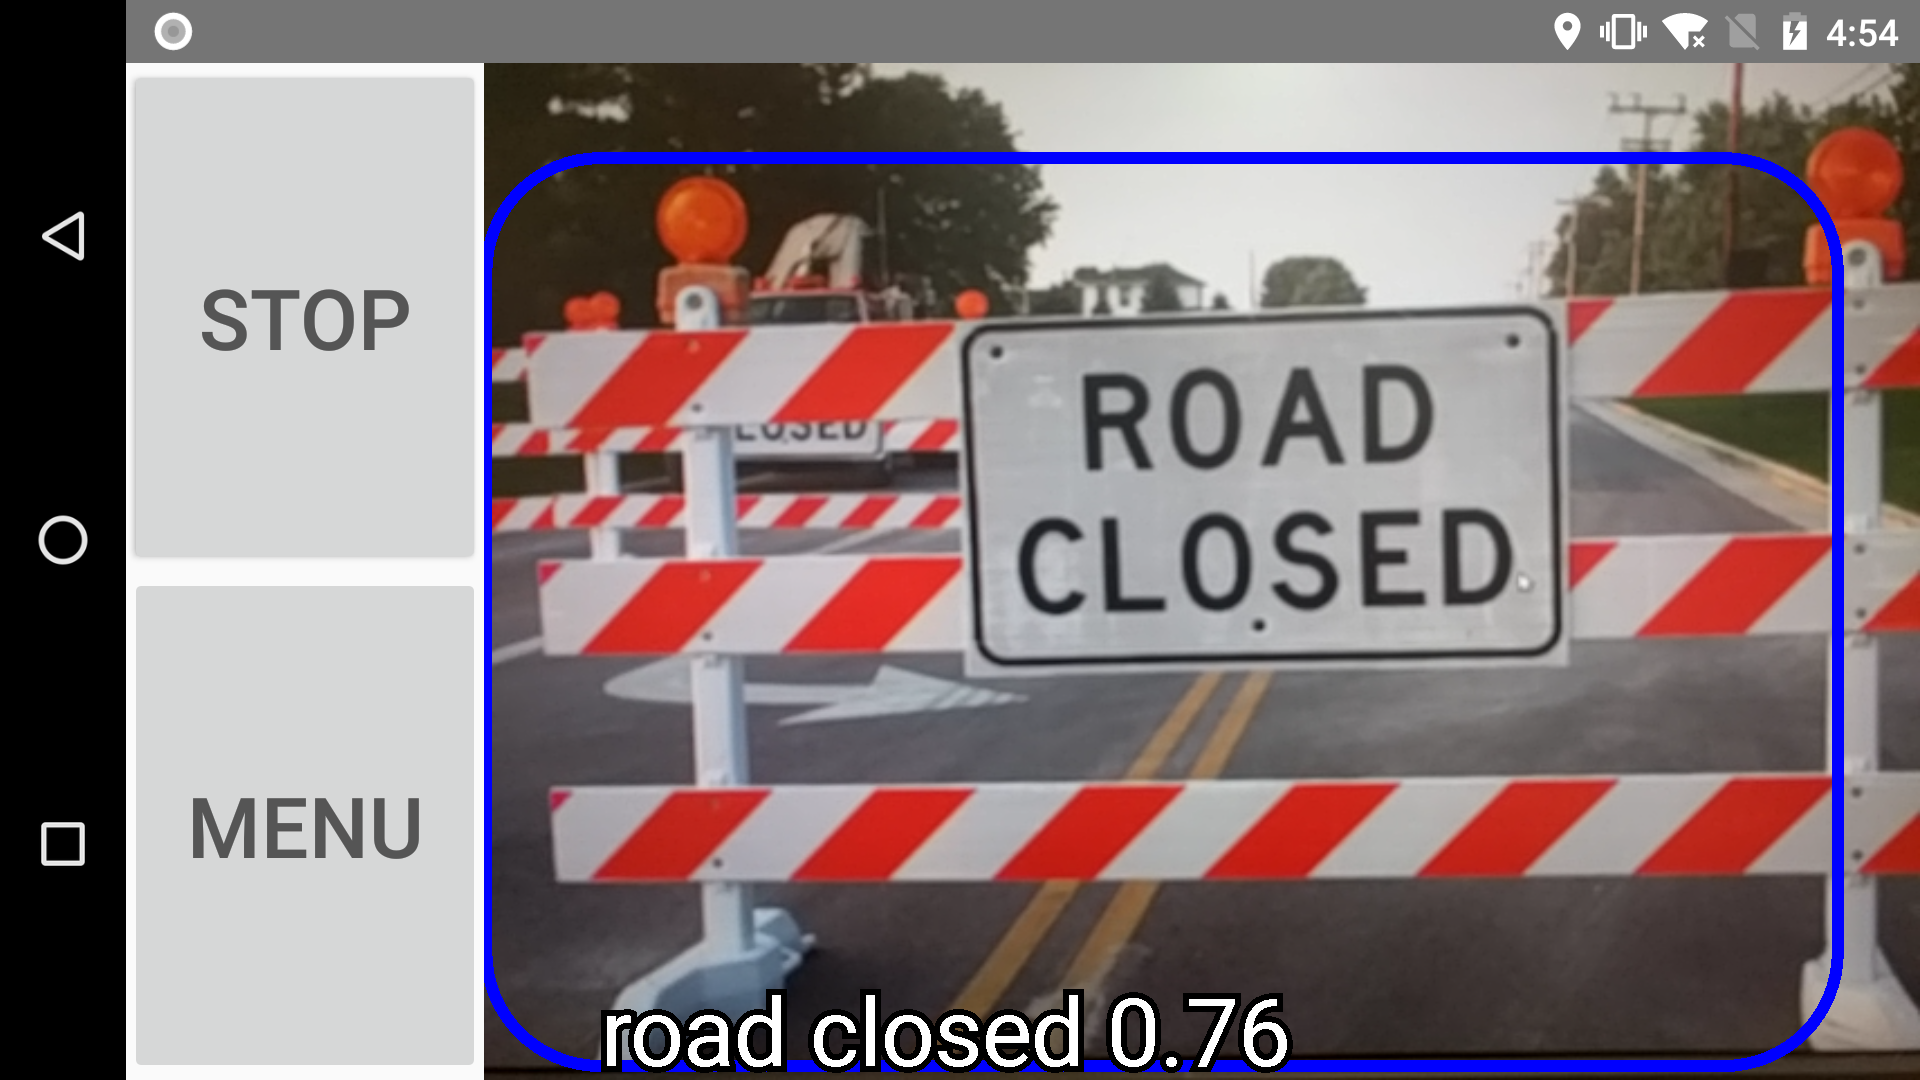
\includegraphics[width=2.6in,angle=0]{Figs/RTDrive/road_closed.png}
\vspace{-0.0cm}
\caption{Road blockage and object detection by TensorFlow in Android Camera Preview mode.}
\vspace{-0.2cm}
\label{road_closed}
\centering
\end{figure}

\begin{figure}[t]
\centering
\vspace{-0.0cm}
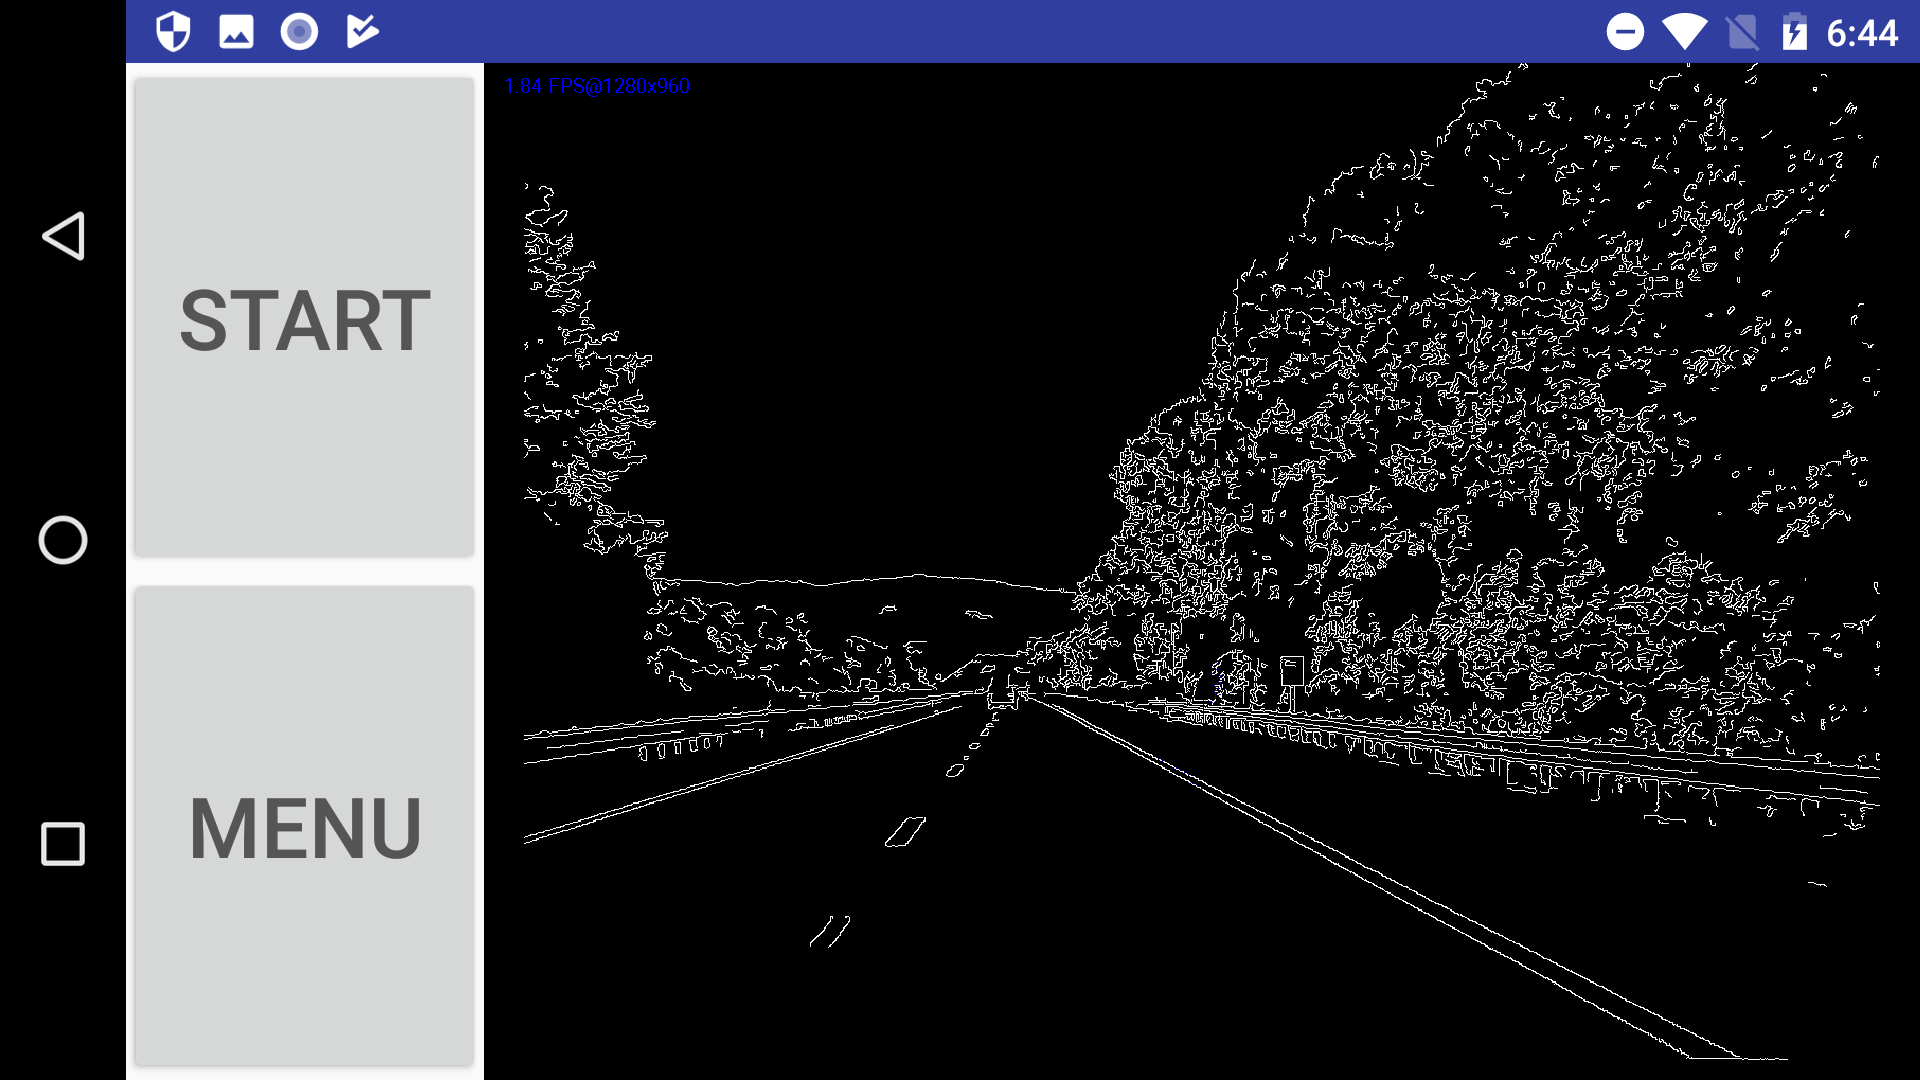
\includegraphics[width=2.6in,angle=0]{Figs/RTDrive/lane_markers.png}
\vspace{-0.0cm}
\caption{Lane marker and road boundary detection by using OpenCV Canny edge detector
in OpenCV preview mode.}
\vspace{-0.2cm}
\label{lane_marker}
\centering
\end{figure}

We use TensorFlow to detect objects and road blockage. 
TensorFlow Core programs consists of two discrete sections, 
building the computational graph and 
running the computational graph \cite{abadi2016tensorflow}.
A computational graph is a series of TensorFlow operations arranged into a graph of nodes. 
In this graph, each node takes zero or more tensors 
as inputs and produces a tensor as an output. 
Nodes in the graph represent mathematical operations, 
while the graph edges represent the multidimensional 
data arrays (tensors) communicated between them. 
Building the computational graph is to use labeled data 
to train the parameters of the graph, 
running the computational graph is to predict the 
outcome given the inputs. 
In our implementation, the computational graph is a blackbox, 
i.e., the input is the image data and 
the output is the identified object. 
We use a prebuilt computational
graph to identify objects and road signs. 
A ``road closed'' sign is identified in Fig. \ref{road_closed}
with a confidential value 0.76 
(higher value means stronger confidence, 1 means the best). 
If such a similar blockage is detected and the self-driving
system cannot handle, the control is transferred to the
remote operator.  
We refer interested
readers to \cite{abadi2016tensorflow, huang2016speed} for detailed graph tranning
and running in TensorFlow.


\subsubsection{Lane Marker and Road Boundary Detection}


We use Canny edge detector, 
Color detector and herustic algorithms to track lane markers and road boundaries. 
Canny edge detector is a multi-stage edge detection
algorithm. 
It uses Gaussian filter to smooth the image in order to remove the noise, 
and then finds the intensity gradients of the image to determine
all possible edges. 
The weak edges are removed if weak or not connected with strong edges. 
Canny edge detector helps us to find the lane and road boundaries. 
To determine the lanes, we use color detector to find all
white and yellow lanes, given the lane markers are either white
or yellow on most roads in US. 
The lane marker and road boundary detection is illusrated in Fig. \ref{lane_marker}. 


\subsubsection{Steering Angle Estimation}

To estimate the steering angle, we use a heuristic algorithm. 
There could be more than one lane in a road segment
and we also need to label the current lane of interest. 
We search from the center of the camera, assuming 
the camera is at the center of the car. 
The first lane markers on both the left side and right side
form the current lane. 
If the lane is straight, then the image view ends at a vanish point
that the lane markers of both side point to. 
The vanish point and the lane markers form a triangle. 
If the lane is curving, then the lane markers of either side
will deviate from this triangle. 
The steering angle is estimated by the coordinates difference
between the triangle and the curved lane markers.   

 }




